%TODO: context-awareness vs. validation (gegenüberstellung)

% Make nice A4 pages for print:
%\usepackage{pgfpages}
%\pgfpagesuselayout{resize to}[a4paper,border shrink=5mm,landscape]

\beamertemplatenavigationsymbolsempty

\setbeamertemplate{bibliography item}[text]

\usepackage[type={CC},modifier={by-sa},version={4.0}]{doclicense}

\usepackage[utf8]{inputenc}
\usepackage{hyperref}
\usepackage{breakurl}
\usepackage{graphicx}
\usepackage{pgfplots}
\usepackage{pgf}
\usepackage{tikz}
\usetikzlibrary{positioning}
\usetikzlibrary{arrows}
\usetikzlibrary{decorations.markings}
\usetikzlibrary{calc}
\usetikzlibrary{matrix}
\usetikzlibrary{shapes}
\usetikzlibrary{decorations.pathmorphing}
\usetikzlibrary{fit}
\usetikzlibrary{backgrounds}
\usetikzlibrary{plotmarks}
\usepackage{stmaryrd}
\usepackage{listings}
\usepackage{pdflscape}
\usepackage{perpage}
\usepackage{appendixnumberbeamer}

%\usepackage[thmmarks,amsmath,amsthm]{ntheorem} % already included in beamer
\usepackage{thm-restate}

\usepackage[sort&compress,numbers]{natbib}  % to be have \citet, \citeauthor, \citeyear

\MakePerPage{footnote}

\tikzstyle{o}=[r,ppBlue]
\tikzstyle{r}=[thick,rectangle,align=center]
\tikzstyle{t}=[r,ppTrans] %,font=\bfseries]
\tikzstyle{dd}=[densely dashed]
\tikzstyle{n}=[r,ppBlue]
\tikzstyle{p}=[r,ppRed]
\tikzstyle{ppRed}  =[draw=red,  fill=  red!20]
\tikzstyle{ppBlue} =[draw=blue, fill= blue!20]
\tikzstyle{ppGreen}=[draw=green,fill=green!20]
\tikzstyle{ppTrans}=[draw=none, fill=none]

\usetheme{Warsaw}

\useoutertheme[subsection=true]{smoothbars}
%\useoutertheme[subsection=false]{miniframes}

\definecolor{bblue}{HTML}{D7DF01}	% yellow-ish actually, for better black/white printing
\definecolor{rred}{HTML}{C0504D}
\definecolor{ggreen}{HTML}{9BBB59}
\definecolor{ppurple}{HTML}{9F4C7C}
\definecolor{lightgray}{rgb}{0.3,0.3,0.3}
\definecolor{lightergray}{rgb}{0.9,0.9,0.9}
\definecolor{UniBlue}{RGB}{83,121,170}

\DeclareTextFontCommand\textintro{\normalfont\bfseries\itshape} % nice!
\newcommand{\intro}[2][]
{%
	\textintro{#2}%
}
\newcommand{\empha}[2][]
{%
	\emph{#2}%
}

%\theoremstyle{plain}
\newcounter{reqcounter}
\newtheorem{requirement}[reqcounter]{Requirement}

%setbeamercolor{structure}{fg=violet}

\makeatletter
\def\th@task{%
    \normalfont % body font
    \setbeamercolor{block title example}{bg=orange,fg=white}
    \setbeamercolor{block body example}{bg=orange!20,fg=black}
    \def\inserttheoremblockenv{exampleblock}
  }
\makeatother

\theoremstyle{task}
\newtheorem{task}{Task}

\newenvironment{assignment}%
{%\setbeamercolor{background canvas}{bg=violet}%
%\setbeamercolor{structure}{fg=cyan!90!black}%
 \setbeamercolor{frametitle}{bg=orange,fg=white}
\begin{frame}}%
{\end{frame}}%

\AtBeginSection[]{
  \begin{frame}
  \vfill
  \centering
  \begin{beamercolorbox}[sep=8pt,center,shadow=true,rounded=true]{title}
    \usebeamerfont{title}\insertsectionhead\par%
  \end{beamercolorbox}
  \tableofcontents
  \vfill
  \end{frame}
}




\pgfplotsset{compat=1.14}
\author{Markus Raab}


\date{5.6.2019}

\begin{document}

\renewcommand{\enquote}[1]{\emph{``#1''}} % Cannot be done earlier

%%%%%%%%%%%%%%%%%%%%%%%%%%%%%%%
\begin{frame}
	\titlepage
	\doclicenseThis
\end{frame}

\begin{frame}
	Lecture is every week Wednesday 09:00 - 11:00.

	\begin{description}
		\item[06.03.2019:] {\color{gray}topic, teams}
		\item[13.03.2019:] {\color{gray}TISS registration, initial PR}
		\item[20.03.2019:] {\color{gray}other registrations, guest lecture}
		\item[27.03.2019:] {\color{gray}PR for first issue done, second started}
		\item[03.04.2019:] {\color{gray}first issue done, PR for second}
		\item[10.04.2019:] {\color{gray}mid-term submission of exercises}
		\item[08.05.2019:] {\color{gray}different location: Complang Libary}
		\item[15.05.2019:]
		\item[22.05.2019:] {\color{gray}all 5 issues done}
		\item[29.05.2019:]
		\item[05.06.2019:] {\color{red}final submission of exercises}
		\item[12.06.2019:]
		\item[19.06.2019:] last corrections of exercises
		\item[26.06.2019:] exam
	\end{description}
\end{frame}

\begin{assignment}
	\frametitle{Tasks for today}
	(until 05.06.2019 23:59)

	\begin{task}
	Submit teamwork and homework.
	\end{task}
\end{assignment}

\begin{frame}
	\frametitle{Popular Topics}
	\vspace{-0.55cm}
	\setlength{\columnsep}{-1.3cm}
	\raggedright
	\definecolor{amethyst}{rgb}{0.6, 0.4, 0.8}
	\begin{multicols}{2}
	\begin{description}
	\item[14] {\color{red} tools}
	\item[9] {\color{gray} testability}
	\item[9] {\color{gray} code-generation}
	\item[7] {\color{amethyst} context-awareness}
	\item[6] {\color{red} specification}
	\item[6] {\color{gray} misconfiguration}
	\item[6] {\color{gray} complexity reduction}
	\item[5] {\color{red} validation}
	\item[5] {\color{gray} points in time} % (early detection)
	\item[5] error messages
	\item[5] {\color{gray} auto-detection}
	\item[4] user interface
	\item[4] {\color{gray} introspection}
	\item[4] {\color{amethyst} design}
	\item[4] {\color{gray} cascading}
	\item[4] {\color{gray} architecture of access}
	\item[3] {\color{gray} configuration sources}
	\item[3] {\color{gray} config-less systems}
	\item[2] secure conf
	\item[2] {\color{gray} architectural decisions}
	\item[1] {\color{red} push vs.\ pull}
	\item[1] {\color{red} infrastructure as code}
	\item[1] full vs.\ partial
	\item[1] convention over conf %iguration
	\item[1] CI/CD
	\item[0] {\color{gray} documentation}
	\end{description}
	\end{multicols}
\end{frame}

\begin{frame}
	\hspace*{-1cm}\includegraphics[width=\paperwidth]{dot/topics}
\end{frame}

\begin{frame}
	\frametitle{Early detection (Recapitulation)}
	\begin{task}
	When do we want to detect misconfiguration?
	\end{task}

	\pause

	Phases when we can detect misconfigurations:
	\begin{itemize} %[<+-| alert@+>]
	\item Compilation stage in configuration management tool
	\item Writing configuration settings on nodes
	\item Starting applications (load-time)
	\item When configuration setting is actually used (run-time)
	\end{itemize}

	\pause[\thebeamerpauses]

	\begin{alertblock}{Problem}
	Earlier versus more context.
	\end{alertblock}
\end{frame}

\begin{frame}
	\frametitle{Cascading (Recapitulation)}

	\begin{task}
	What is cascading configuration?
	\end{task}
	\vspace{1em}

	\pause

	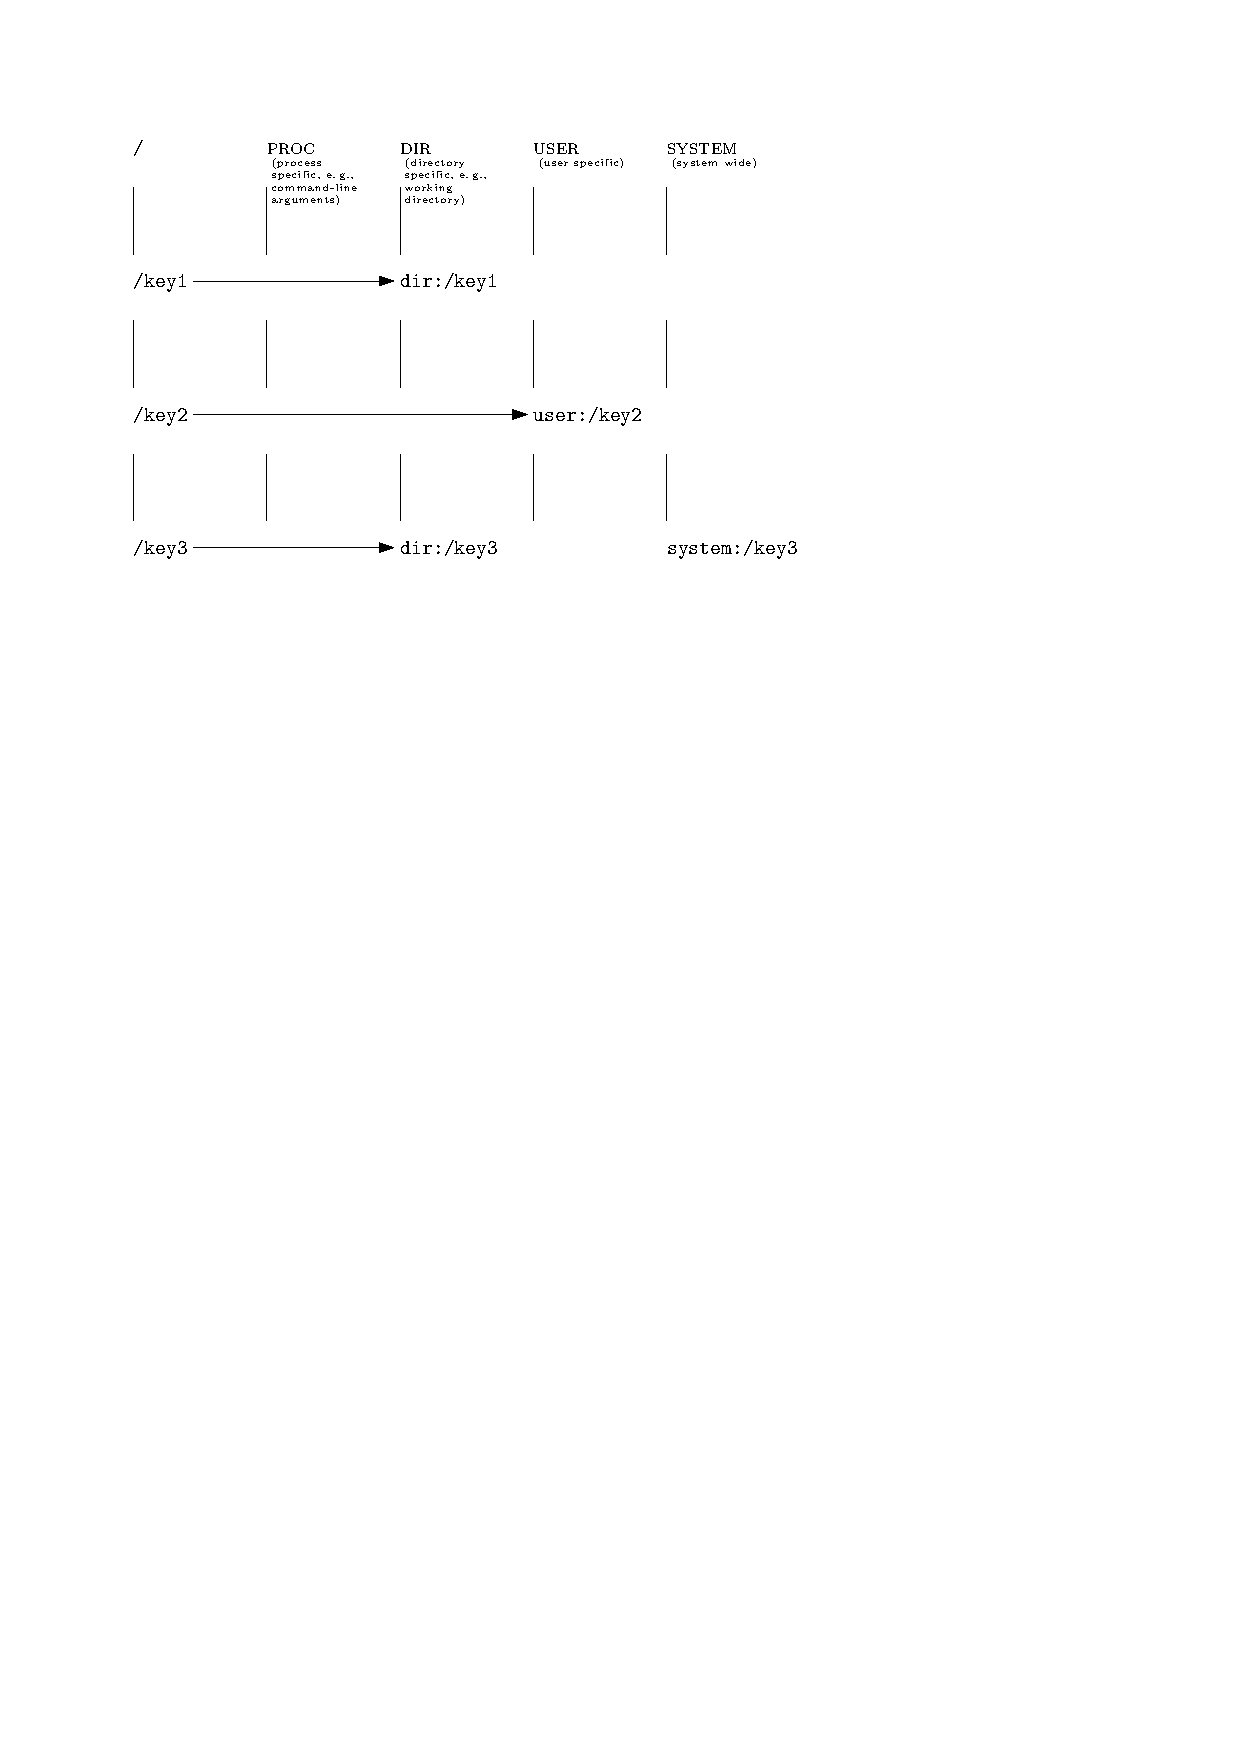
\includegraphics[scale=0.7]{cascading}
\end{frame}

\begin{frame}
	\frametitle{Contextual Values (Recapitulation)}

	\begin{task}
	What are contextual values?
	\end{task}

	\pause

	\ExecuteMetaData[../book/background.tex]{contextual-values}
\end{frame}

\begin{frame}
	\frametitle{Definition Context (Recapitulation)}

	\begin{task}
	What is context-aware configuration?
	\end{task}

	\pause

	\ExecuteMetaData[../book/background.tex]{context-definition}
\end{frame}

\begin{frame}
	\frametitle{Elektra (Recapitulation)}

	\pause

	\begin{itemize}
	\item is not only a key database but a specification language to describe a key database
	\item plugins implement the specification (could be distributed but focus is configuration files)
	\item is library based (no single point of failure, no distributed coordination needed)
	\item supports transactions (persisting whole KeySets at once)
	\item supports integration of existing configuration settings
	\end{itemize}
\end{frame}

%%%%%%%%%%%%%%%%%%%%%%%%%%%%%%%%%%%%%%%%%% 
\section{Terms and Properties}

\subsection{}

\begin{frame}
	\frametitle{Definition Configuration Management (Recapitulation)}

	\pause

	\begin{itemize}
	\item is a discipline in which configuration (in the broader sense) is administered.
	\item makes sure computers are assembled from desired parts and the correct applications are installed.
	\item has means to describe the desired configuration of the whole managed system.
	\item ensures that the execution environment of installed applications is as required.
	\end{itemize}
\end{frame}

\begin{frame}
	\frametitle{Possible Benefits of CM (Recapitulation)}

	\pause

	\begin{itemize} %[<+-| alert@+>]
	\item All advantages scripts have: \\
		Documentation, Customization, Reproducability
	\item Declarative description of the system \\
		(Infrastructure as Code~\cite{waldemar2013testing})
	\item Auditability
	\item Less configuration drift
	\item Error handling
	\item Pull/Push
	\item Reusability
	\item (Resource) Abstractions
	\end{itemize}
\end{frame}

\begin{frame}
	\frametitle{Infrastructure as Code}

	Once we described configuration settings,
	configuration settings are simply an instantiation of the configuration specifications.
	\vspace{1em}

	Code describing the instantiation is \textbf{CM code}.
	\vspace{1em}

	\textbf{Auditability:}
	Being informed about status and changes in the infrastructure.
	\vspace{1em}

	\begin{alertblock}{Goal}
	Single Source of Truth
	\end{alertblock}
\end{frame}

\begin{frame}
	\frametitle{Configuration Drift}

	Are derivations of the ``Single Source of Truth'' (the CM code).

	Caused by:

	\pause

	\begin{itemize}[<+-| alert@+>]
	\item manual configuration changes by administrators
	\item manual configuration changes by end users
	\item differences in updates (e.g., skipped or failed updates)
	\item failed attempts to change configuration
	\item applying different versions of CM code
	\item \dots
	\end{itemize}
\end{frame}

\begin{assignment}
	\begin{task}
	Break.
	\end{task}
\end{assignment}

\begin{frame}
	\frametitle{Push vs.\ Pull}

	\begin{itemize}[<+-| alert@+>]
	\item Push is more interactive.
	\item Push cannot do its job if nodes are not reachable.
	\item Push needs additional techniques to scale with many nodes.
	\item Push demands access to servers from a single server.
	\item Pull needs additional monitoring to know when a patch has been applied.
	\item Pull needs resources even if nothing is to do.
	\end{itemize}

	\begin{task}
	Do you prefer push or pull?
	What does your CM tool of choice use?
	\end{task}
\end{frame}


\begin{frame}
	\frametitle{Idempotence}

	idem + potence (same + power)
	\vspace{2em}

	Yield same result with any number of applications ($n\ge1$):
		
	\[
		f(f(x))=f(x)
	\]
\end{frame}


\begin{frame}
	\citet{wadler2003xml} describe two further properties:
	\vspace{2em}

	\begin{description}
	\item[Self-describing]
	means that from the configuration file alone we are able to derive the correct internal representation.

	\item[Round-tripping]
	means that if a data-structure (e.g., KeySet) is serialized and then parsed again, we end up with an identical internal representation.
	\end{description}

	\pause

	\vspace{2em}
	Round-tripping is a prerequisite of idempotence.

	\pause

	\begin{task}
	Explain the three concepts your neighbor (idempotence, self-describing, round-tripping).
	\end{task}
\end{frame}


%%%%%%%%%%%%%%%%%%%%%%%%%%%%%%%%%%%%%%%%%% 
\section{Validation}

\subsection{}

%Describe constraints in OOP (Babelsberg)?

\begin{frame}
	\frametitle{Goals}

	Checking the specifications vs.\ checking the settings.

\end{frame}

\begin{frame}
	\frametitle{Checking Configurations}

	Following properties of configuration settings can be checked:

	\begin{itemize}[<+-| alert@+>]
	\item structure
	\item values (data types)
	\item constraints
	\item semantic checks (e.g., IP, folder)
	\item domain-specific checks (e.g., databases)
	\item requirements (suitable configurations)
	\item context (context-aware configurations)
	\end{itemize}
\end{frame}

\begin{frame}[allowframebreaks]
	\frametitle{}
	\elektra{} supports many other data types, each implemented in its own plugin(s):
	\begin{description}
	\item [check/type] allows us to specify CORBA data types.
	Checking ``any'' (default) is always successful.
	The record and enum types defined by CORBA are not part of this plugin but of others as explained below.

	\item [check/enum] supports a list of supported values denoted by array indexes.
	\item [check/bool] transforms specific strings, for example ``true'' and ``false'', into the canonical boolean representation, i.\,e., ``0'' and ``1''.
	\item [check/ipaddr] checks if a string is a valid IP address.
	\item [check/path] checks presence, permissions, and type of paths in the file system.
	\item [check/date] supports to check date formats such as POSIX, ISO8601, and RFC2822.
	\item [check/validation] checks the configuration value with regular expressions.
	\item [check/condition] checks using conditionals and comparisons.
	\item [check/math] checks using mathematical expressions.
	\item [check/range] allows us to check if numerical values are within a range.
	\item [trigger/error] allows us to express unconditional failures.
	\end{description}
\end{frame}

\begin{frame}
	\frametitle{Checking Specifications}

	The goals of checking \elektra{Spec} are:

	\begin{itemize}[<+-| alert@+>]
	\item Defaults must be present for safe lookups.
	This goal also implies that there must be at least one valid configuration setting.
	\item Types of default values must be compatible with the types of the keys.
	\item Every contextual interpretation of a key must yield a compatible type.
	\item Links must not refer to each other in cycles.
	\item Every link and the pointee must have compatible types.
	\end{itemize}
\end{frame}

\begin{frame}[fragile]
	\frametitle{Example}

	\begin{code}[morekeywords={override},gobble=4]
	[sw/org/abc/has_true_arg]
	  type:=boolean
	  default:=0
	  override/#0:=/sw/org/abc/arg0
	  override/#1:=/sw/org/abc/arg1
	\end{code}
\end{frame}

\begin{frame}[fragile]
	\frametitle{Logfile Example}

	\begin{code}[morekeywords={path},gobble=4]
	[slapd/logfile]
	  check/path:=file
	\end{code}
\end{frame}

\begin{frame}[fragile]
	\frametitle{Logfile Extensions}

	\begin{code}[morekeywords={match,path},gobble=4]
	[slapd/logfile]
	  check/path:=file
	  check/validation:=^/var/log/
	  check/validation/message:=Policy violation:
	    log files must be below /var/log
	\end{code}
\end{frame}

\begin{frame}[fragile]
	\frametitle{Error Messages}

	Error messages are extremely important as they are the main communication channel to system administrators.\\
	Example specification:
	\vspace{1em}

	\begin{code}[morekeywords={assign,math},gobble=4]
	[a]
	  check/type:=long
	[b]
	  check/type:=long
	[c]
	  check/range:=0-10
	  assign/math:=../a+../b
	\end{code}
\end{frame}

\begin{frame}[fragile]
	\frametitle{Error Messages}

	Problems:
	\begin{itemize}[<+-| alert@+>]
	\item Generic vs.\ specific plugins
	\item General principles of good error messages~\cite{lee2011personifying}
	\item Give context
	\item Precisely locate the cause:
	\end{itemize}
	\vspace{1em}

	\pause[\thebeamerpauses]

	\begin{code}[language=CfgElektra,gobble=4]
	a=5  ; unmodified
	b=10 ; modification bit in metadata
	     ; is only set here
	c=15 ; unmodified by user but changed
	     ; later by assign/math
	\end{code}
\end{frame}

\begin{frame}[fragile]
	\frametitle{Example Error Messages}
\begin{verbatim}
Sorry, I was unable to change the configuration settings!
Description: I tried to set a value outside the range!
Reason: I tried to modify b to be 10 but this caused c to
        be outside of the allowed range (0-10).
Module: range
At: sourcefile.c:1234
Mountpoint: /test
Configfile: /etc/testfile.conf
\end{verbatim}
\end{frame}


\begin{frame}
	\frametitle{Conclusion}

	\begin{itemize}[<+-| alert@+>]
	\item Definition and challenges in configuration management.
	\item Properties: self-describing, idempotent, round-tripping.
	\item Validation is combined effort of devs and admins.
	\end{itemize}
\end{frame}


\begin{frame}
	\frametitle{Outlook}

	\begin{itemize}[<+-| alert@+>]
	\item Configuration Management Tools and Languages
	\item Error Messages
	\item User View of Administrators
	\end{itemize}
\end{frame}




%%%%%%%%%%%%%%%%%%%%%%%%%%%%%%%%%%%%%%%%%% 
\nocite{raab2017introducing}

\appendix

\begin{frame}[allowframebreaks]
	\bibliographystyle{plainnat}
	\bibliography{../shared/elektra.bib}
\end{frame}

\end{document}

